\begin{sidewaysfigure*}
\thisfloatpagestyle{mylandscape}%
\rotatesidewayslabel%
\centering

\begin{subfigure}[t]{0.32\textwidth}
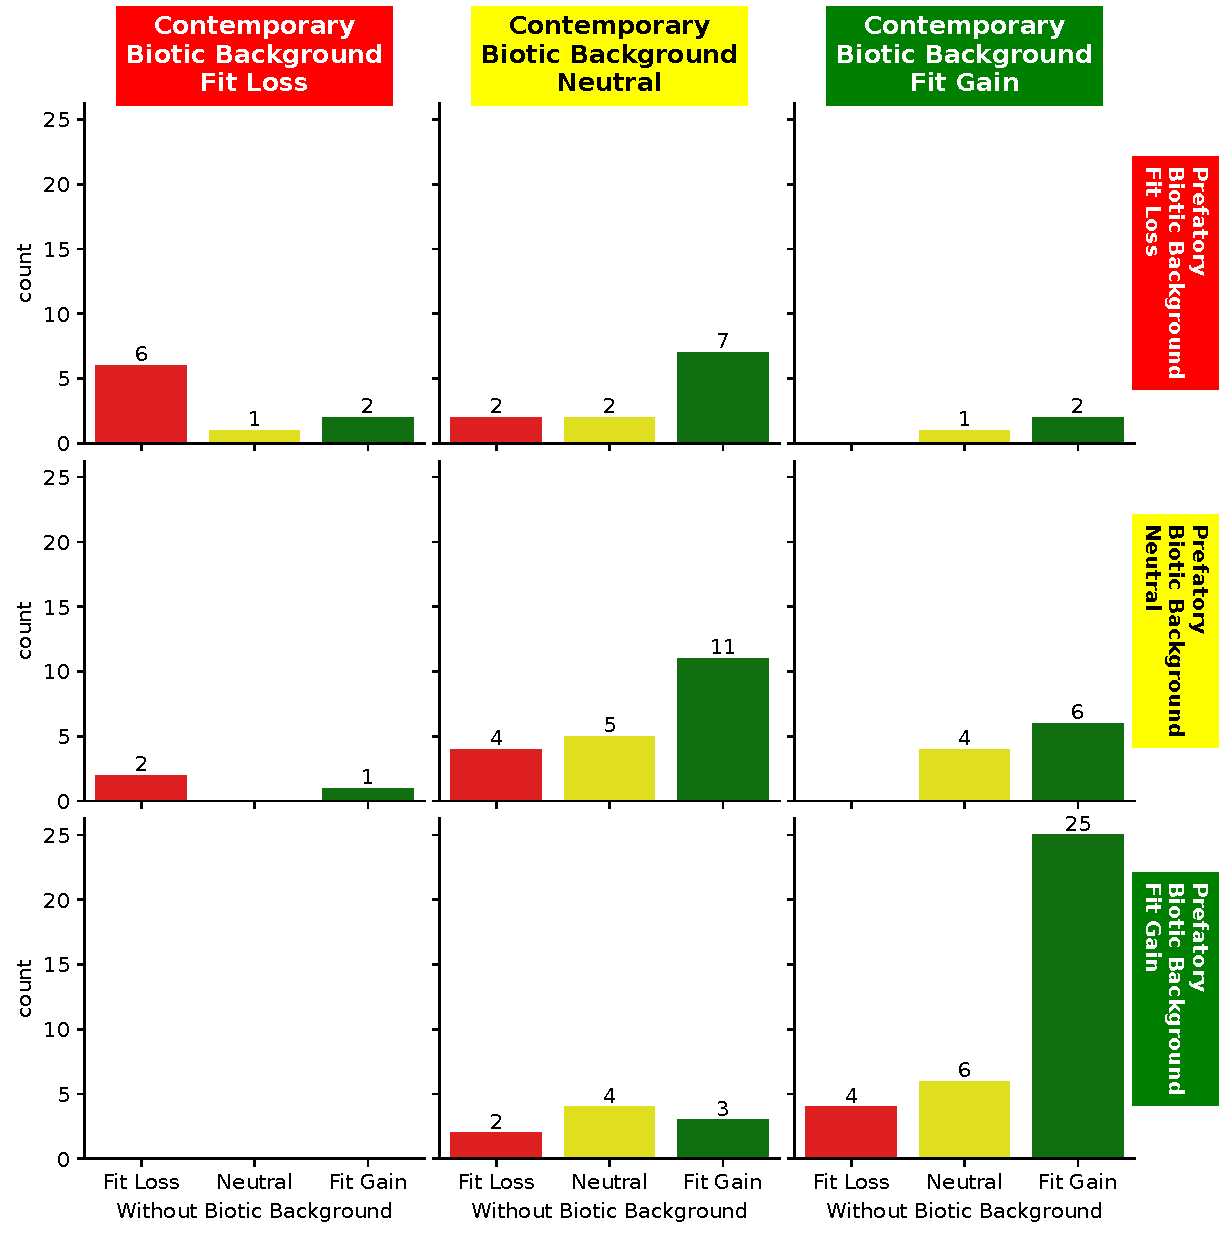
\includegraphics[width=\linewidth]{{submodule/dishtiny/binder/bucket=prq49/a=adaptation_assays+endeavor=16/teeplots/assay-subject=Specimen+col=contemporary-biotic-background+kind=count+row=prefatory-biotic-background+viz=barlabel-catplot+x=without-biotic-background+ext=}}
\caption{Joint distribution of adaptation assay on representative specimen from focal strain over biotic backgrounds, with diversity maintenance during competition.}
\label{fig:outcome_count_joint_distns:specimen_with_dm}
\end{subfigure}%
\hfill%
\begin{subfigure}[t]{0.32\textwidth}
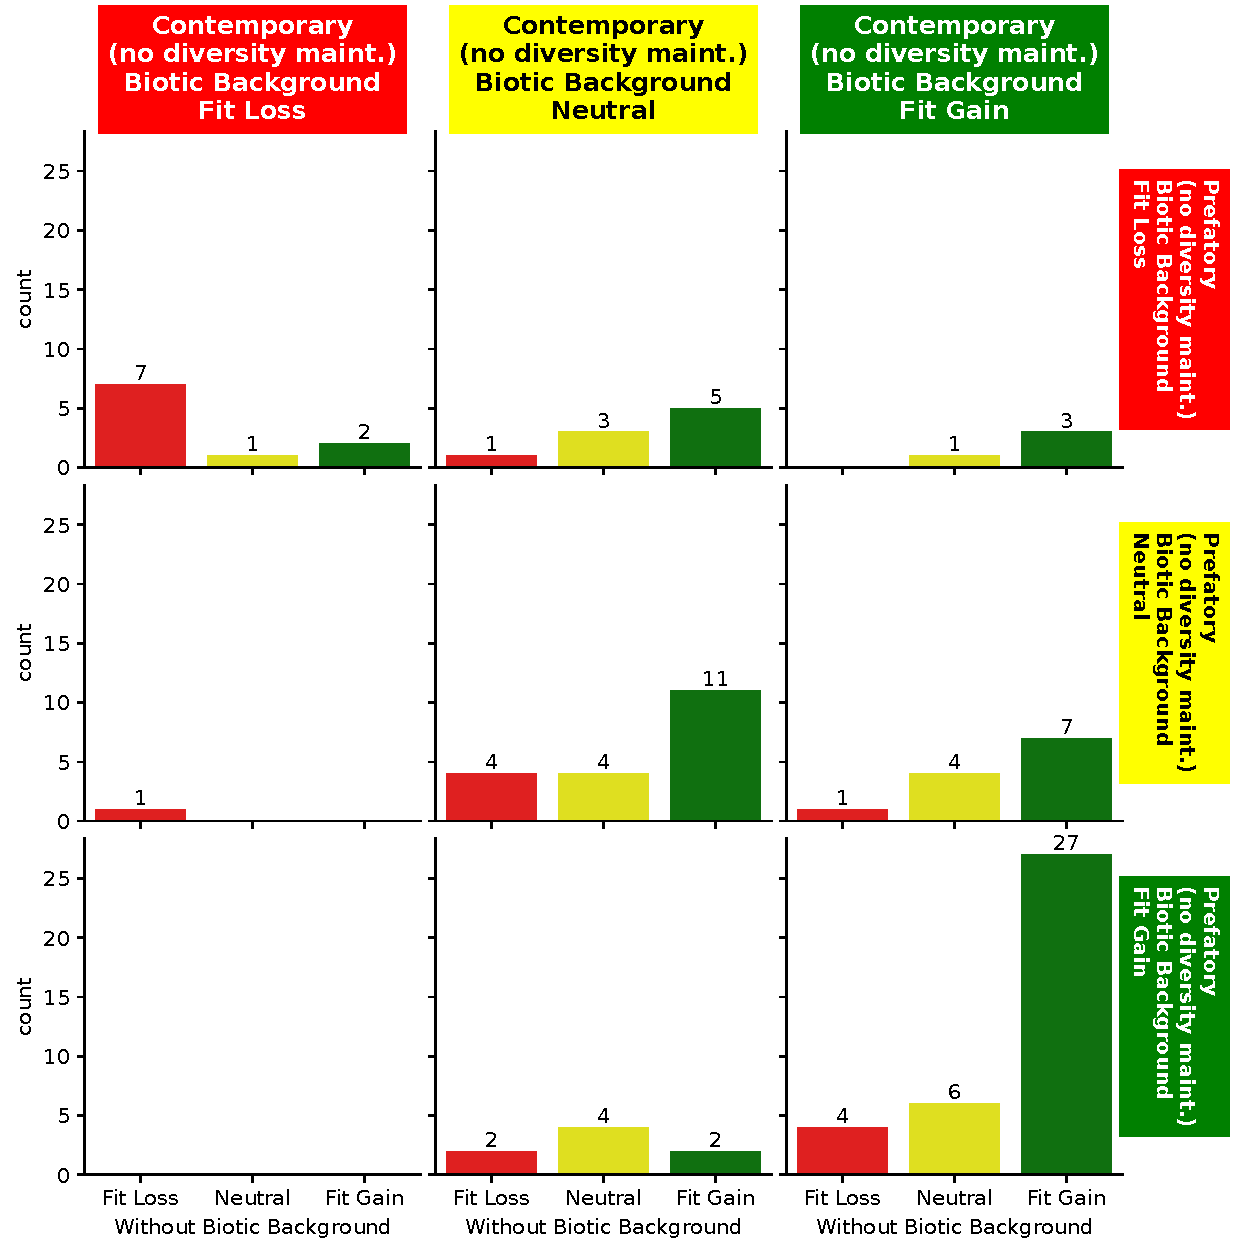
\includegraphics[width=\linewidth]{{submodule/dishtiny/binder/bucket=prq49/a=adaptation_assays+endeavor=16/teeplots/assay-subject=Specimen+col=contemporary-no-diversity-maint-biotic-background+kind=count+row=prefatory-no-diversity-maint-biotic-background+viz=barlabel-catplot+x=without-biotic-background+ext=}}
\caption{Joint distribution of adaptation assay on representative specimen from focal strain over biotic backgrounds, with diversity maintenance disabled during competition.}
\label{fig:outcome_count_joint_distns:specimen_no_dm}
\end{subfigure}%
\hfill%
\begin{subfigure}[t]{0.32\textwidth}
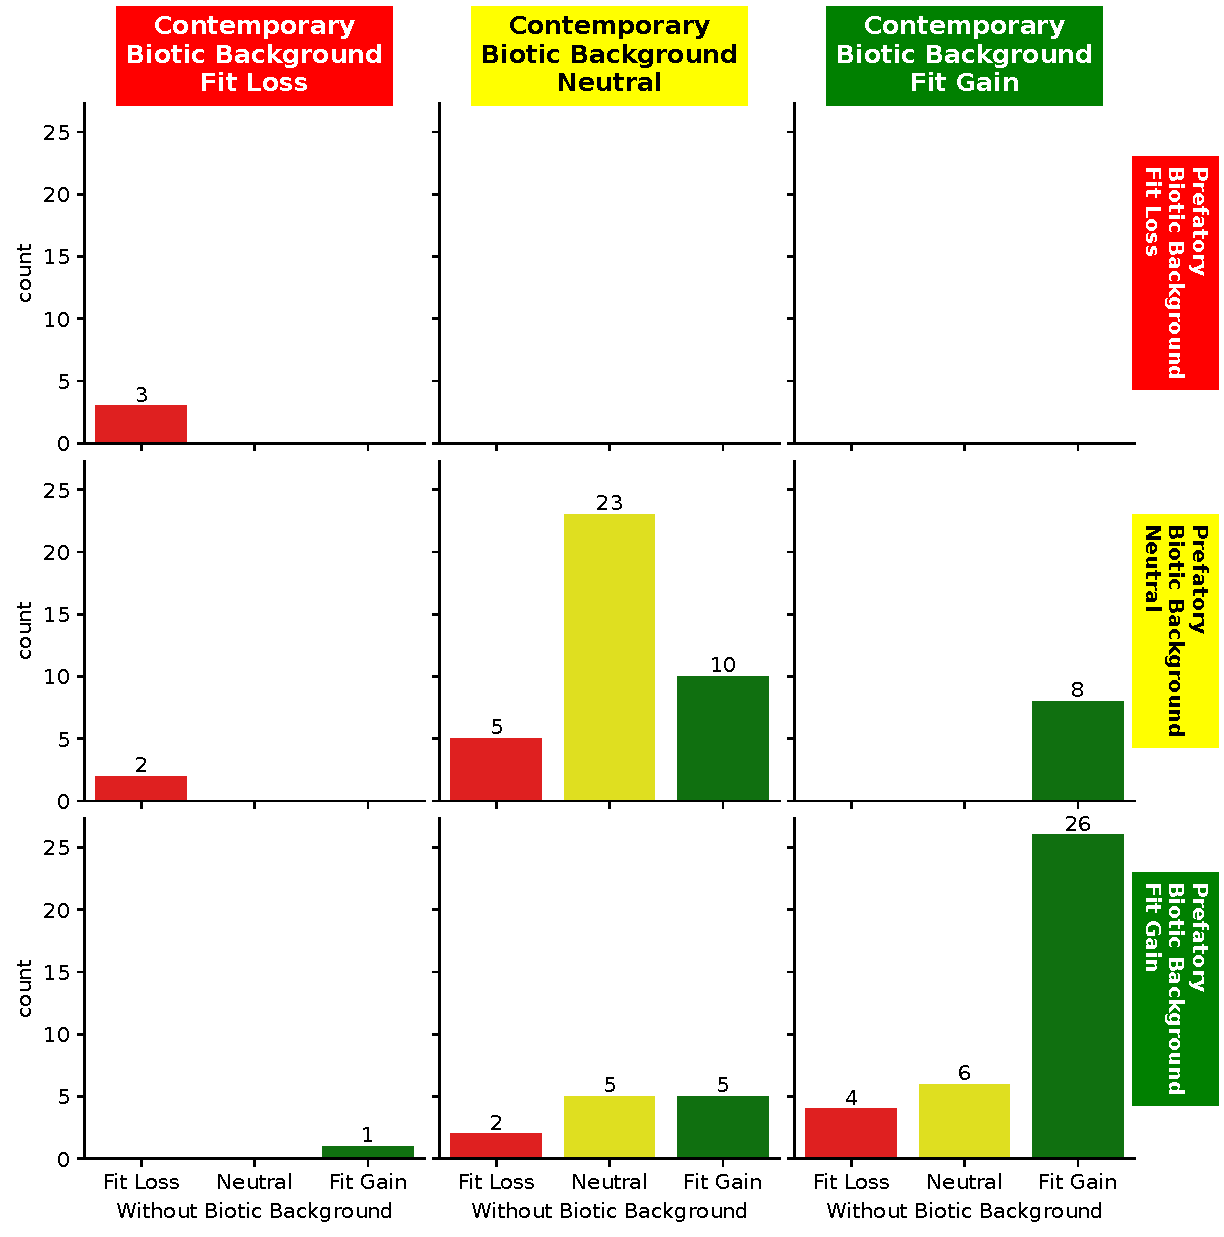
\includegraphics[width=\linewidth]{{submodule/dishtiny/binder/bucket=prq49/a=adaptation_assays+endeavor=16/teeplots/assay-subject=Population+col=contemporary-biotic-background+kind=count+row=prefatory-biotic-background+viz=barlabel-catplot+x=without-biotic-background+ext=}}
\caption{Joint distribution of adaptation assay on focal strain population over biotic backgrounds, with diversity maintenance during competition.}
\label{fig:outcome_count_joint_distns:population}
\end{subfigure}


\caption{
\textbf{Effect of biotic background on adaptation assay outcomes.}
\footnotesize
Joint distribution of adaptation assay outcomes across biotic backgrounds.
For each adaptation assay, three outcomes were possible: significant fitness gain, significant fitness loss, or no significant fitness change (``neutral'').
Significance cutoff $p < 0.005$ was used.
A fitness loss --- color-coded red --- corresponds to winning 2 or fewer competitions out of 20 against the preceding stint's focal strain population.
A fitness gain --- color-coded green --- corresponds to winning 18 or more competitions out of 20 against the preceding stint's focal strain population.
Neutral fitness outcomes are color-coded yellow.
Outcome counts are accumulated over experiments from stint 1 through stint 100.
Counts in each subfigure therefore sum to 100.
Column position in facet grid indicates outcome with contemporary biotic background, row position indicates outcome with prefatory biotic background, and bar color and $x$ position indicates outcome without biotic background.
See Figure \ref{fig:adaptation_assay_cartoon} for explanation of competition biotic backgrounds.
See Figure \ref{fig:with_vs_without_diversity_maintenance} for detail on joint distribution of outcomes with and without diversity maintenance, which were mostly identical.
}
\label{fig:outcome_count_joint_distns}
\end{sidewaysfigure*}
